\chapter{Diseño e implementación del servidor}

En este capítulo abarcaremos todo lo circundante al diseño e implementación del servidor, describiendo cada servicio de forma particular.

    [Incluir imagen de usted esta aqui basada en el esquema del sistema general version final].

\section{Actualidad del desarrollo web}

En la web existen dos grandes mundos, el frontend el cual es la parte de la web con la que interactuan los usuarios o clientes. Por otro lado tenemos al Backend que es la parte que se conecta con la base de datos y ejecuta las validaciones necesarias para leer o escribir información. En general, el frontend y el backend suelen ser 2 proyectos separados y pueden ser construidos en diferentes lenguajes. Los lenguajes más utilizados son: JavaScript (JS), Python, Ruby, entre otros \cite{presta_10_2021}.

Hoy en día la web se a transformado en la base de cualquier organización, hace años las organizaciones solian usar aplicaciones de escritorio, pero en la actualidad las aplicaciones web han ganado el mercado.
De este estandar de implementar aplicaciones en forma de webs, nace la necesidad de desacoplar los servicios de una web en partes más pequeñas, lo que se denomina microservicios y suelen correr en lo que se llama una red de contenedores, usualmente bajo Docker \cite{docker_inc_documentacion_2023}.

La principal ventaja de la arquitectura de microservicios es la independecia de tecnologías, siendo posible implementar sistemas en lenguajes muy diversos, por ejemplo, los sistemas de recomendación o reconocimiento suelen estar implementados en Python debido a la gran cantidad de librerias de analisis de datos desarrolladas para este lenguaje. Pero por otro lado servicios relacionados a la busqueda y clasificación de informacion pueden ser implementados en Javascript, Ruby, o Go, entre otros.

\section{Qué es un servicio?}

Un servicio se puede entender como una aplicación desarrollada para cumplir una serie de tareas. Existen una gran diversidad de tipos de servicios, tales como bases de datos, sistemas de recomendación, aplicaciones backend, paginas webs, brokers MQTT, etc. Los servicios suelen establecer interfaces de comunicación, para que los otros servicios o aplicaciones que se conecten sepan donde deben pedir la información y que van a recibir.

\section{Docker}

Docker es una tecnología open source desarrollada por Docker Inc, la cual permite correr servicios de forma aislada en contenedores. Un contenedor funciona casi como una maquina virtual, pero sin entorno gráfico y compartiendo el Kernel \cite{keepcoding_que_2022} con el sistema que lo hospeda, lo que hace que los contenedores sean más livianos y mucho más rapidos que una maquina virtual, ya que estan últimas emulan todo el sistema e incluyen un puente entren el kernel del sistema padre y el sistema emulado.

Docker al ser una tecnología muy versatil posee una gran cantidad de herramientas que lo rodean, la más conocida, y muy utilizada en el mundo del desarrollo es Kubernetes [cita a kubernetes]. Debido a que el sistema no es lo suficientemente grande y se cuenta con multiples servidores para alojar los servicios, se implementaron utilizando Docker compose \cite{docker_inc_docker_2023}, el cual cumple un rol muy similar a Kubernetes, pero sin tanta complejidad extra que trae la opción de administrar multiples servidores.

Docker compose genera una red interna para interconectar los contenedores, lo que conlleva a un contenedor de nombre \textit{api} pueda acceder a una base de datos montada en un contenedor con el nombre \textit{db} utilizando como nombre de dominio la palabra \textit{db} junto con el puerto correspondiente, en caso de bases de datos Mongo el puerto por defecto es el 27017, en dicho caso la url de conexión queda dada como \textit{``mongodb://db:27017/database"}.

\section{Servicios}

Una vez descripta como es la arquitectura actual de las aplicaciones web, y que sabemos que es Docker pasaremos a explicar en profundidad de cada servicio y sus usos, junto con cada tecnología aplicada. La arquitecura del servidor se puede observar en la Fig. \ref{fig:server-esquema} junto con el flujo simplificado de información.

\begin{figure}
    \centering
    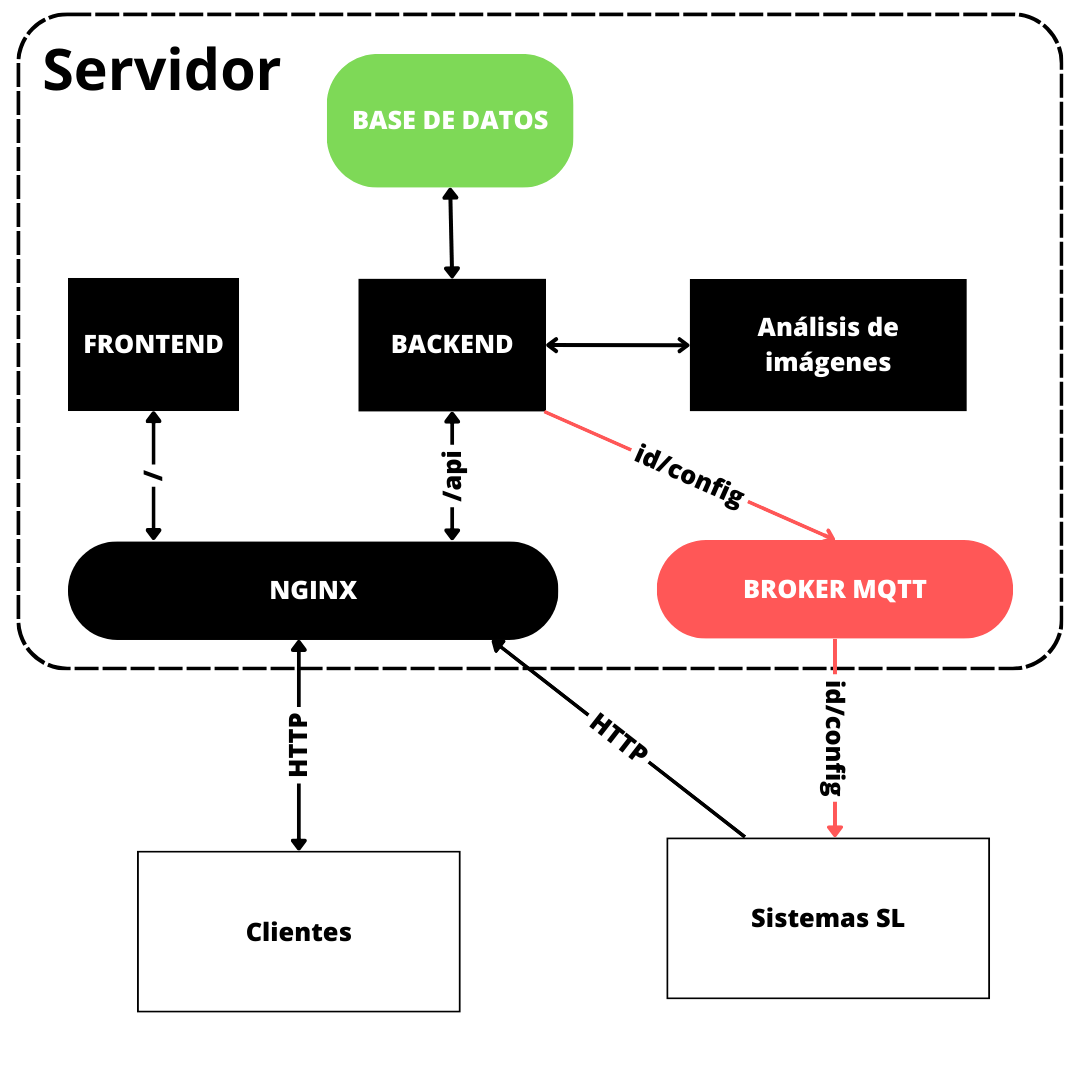
\includegraphics[width=.8\textwidth]{imgs/server-esquema.png}
    \caption{Esquema del servidor junto con la conexión de clientes y barreras.}
    \label{fig:server-esquema}
\end{figure}

\subsection{Base de datos}

La base de datos elejida fue Mongo DB [documentacion de mongo], debido a que una de las bases de datos más utilizadas en el mundo basada en documentos. Mongo almacena los datos en un formato denominado BSON (binary JSON), le cual hace más fácil la transferencia de datos. Por otro lado, nos permite escalar de forma horizontal de forma mucho más sencilla, ya que se suelen usar identificadores únicos y no incrementales, como es frecuente en bases de datos sequenciales.

El esquema de base de datos [figura de la base de datos].

\subsection{Broker MQTT}

Debido a que Mosquitto es el broker MQTT más utilizado, el cual utiliza la versión 5.0 del protocolo. Elúnico tópico implementado en el de configuración de las barreras, este tópico tiene la forma de ``\textit{id}/config" donde \textit{id} es el id único de la barrera, esto permite de que existan tantos tópicos como barreras, y solo pueden escuchar los cambios de configuracíón de ellas, lo que permite ahorrar procesamiento de datos en la barrera.

\subsection{Backend}

Existen 2 aplicaciones Backend, la principal fue escrita en NestJS \cite{noauthor_documentacion_nodate} la cual se encarga de conectarse con la MongoDB, el Backend de Python y escucha las peticiones del frontend y de las barreras, la segunda es el Backend de Python, el cual ejecuta el algoritmo de OCR.

El servicio de NestJS, fue implementado junto con Swagger [cita  a la documentacion de swagger], lo que genera documentación de los endpoints HTTP de forma automatica, facilitando la tarea de agregar más personas al proyecto y poder visualizar información necesaria por los endpoints para su llamada, además de mostrar el verbo HTTP con el que se debe llamar el mismo [agregar figura de swagger]. Un eje fundamental a la hora de implementar este servicio, fue la seguridad, es por ello que se utilizo PassportJS [cita a documentacion de passport], en sintesis, esta librerira permite implementar métodos de autenticación de forma facíl y sencilla, en este proyecto se implementaron los siguientes métodos:

\begin{enumerate}
    \item Usuario y contraseña: Utilizado principalmente para los usuarios que entran/registran desde la web.
    \item ApiKey de terceros: Una forma de validar si la aplicación que pide datos esta autorizada o no.
    \item ApiKey para barreras: Permite validar si la información del registro de entrada/salida esta siendo enviada por una barrera autorizada, además nos permite saber que barrera es la que envia los datos.
    \item Json Web Token o JWT: Se utiliza una vez que el usuario entra a la app, y es un hash generado por el servidor, los tokens poseen un tiempo de vida, en nuestro caso 1 día.
\end{enumerate}

{\huge no sabemos que hablar del backend, deberiamos poner algo de los endpoints?}

El servicio de Python, es una API implementada con Flask [documentacion de flask], este servicio recibe una fotografía y la procesa utilizando el algoritmo de OCR descripto en el capítulo 2 para devolver la patente.

\subsection{Frontend}

El frontend fue construido enterament en ReactJS [documentacion de React], la cual es una de las librerias de JavaScript más utilizadas en la industria. La idea principal de este servicio es brindar un centro de control de las barreras, y visualización de registros y datos de interes. Además permite a los administradores crear barreras, y ver el estado de las mismas.

\subsubsection*{Pagínas para los usuarios}

Los usuarios puede registrarse y entrar a la plataforma como se ve en [referencia a figura de login y registro]. Luego del entrar pueden visualizar los estacionamientos que ellos poseen [figura del home], además de poder configurar los parametros de las barreras en tiempo real [figura de la configuracion de las barreras]. Los ususarios cuentan con un dashboard que les permite ver información resumida por el momento pueden ver horas estacionadas y vehiculos estacionados, separados por estacionamiento y visulizando el tiempo por día, mes o año [figura del dashboard].

\subsubsection*{Pagínas para los administradores}

Los administradores poseen una pagina para visualizar las barreras según lugar, permitiendo un prefiltado según clientes lo que hace más sencillo encontrar alguna barrera [figura de la pagina]. Por último, poseen una pagína para agregar barreras a un lugar [figura del form de agregar barrreras].

\subsection{Nginx}

Nginx es un servido web de código abierto que permite la implementación de proxy inverso, cache de HTTP, y balanceo de cargo, además de contar con una facíl configuración [documentacion de nginx].
En este caso, la implementación de Nginx se utiliza para que la aplicación backend de NestJS y el frontend esten corriendo en la misma IP, es decir, se utiliza la configuración de proxy inverso.